\part{Кратні інтеграли на гіперпрямокутниках}\label{part:boxes}
\chapter{Теоретичні відомості}
\section{Означення}
\begin{definition}[Гіперпрямокутник]\index{гіперпрямокутник}\label{def:box}
Нехай $m$ --- натуральне число, ${a_1<b_1}$, ${a_2 < b_2}$, $\ldots$, ${a_m < b_m}$ --- фіксовані дійсні числа. Будемо називати ($m$--вимірним) гіпркпрямокутником або брусом декартів добуток
\[
Q = \segment{a_1}{b_1}\times\segment{a_2}{b_2}\times\ldots\times\segment{a_m}{b_m} \subset \eucl{m},
\]
тобто множину таких елементів ${\left(x_1, x_2, \ldots, x_m\right)}$ з евклідового простору \eucl{m}, координати яких задовольняють нерівності
\[
\begin{array}{cccc}
a_1\leq x_1\leq b_1,&
a_2\leq x_2\leq b_2,&
\ldots,&
a_m\leq x_m\leq b_m.
\end{array}
\]
Мірою $Q$ будемо називати наступне число
\[
\m(Q) = \left(b_1-a_1\right)\left(b_2 - a_2\right)\ldots\left(b_m-a_m\right) = \prod\limits_{j=1}^{m}\left(b_j - a_j\right).
\]
\end{definition}
\begin{example}
Частинними випадками брусів є
\begin{itemize}
\item одновимірний брус --- відрізок ${\segment{a}{b}\subset\R}$;
\item двовимірний брус --- прямокутник ${\segment{a_1}{b_1}\times\segment{a_2}{b_2}\subset\eucl{2}}$;
\item тривимірний брус --- прямокутний паралелепіпед  ${\segment{a_1}{b_1}\times\segment{a_2}{b_2}\times\segment{a_3}{b_3}\subset\eucl{3}}$.
\end{itemize}
\end{example}
Нагадаємо означення розбиття відрізку (одновимірного брусу), яке вивчається в темі "Визначений інтеграл Рімана".
\begin{definition}[Розбиття відрізку]
Розбиттям відрізку \segment{a}{b} називають набір чисел ${\left\{t_0, t_1, t_2, \ldots, t_{n-1}, t_{n}\right\}}$, які задовольняють умови
\[
a = t_0 < t_1 < t_2 < \ldots  < t_{n-1} < t_{n} = b.
\]
При цьому відрізки \segment{t_0}{t_1}, \segment{t_1}{t_2}, ${\ldots}$, \segment{t_{n-1}}{t_{n}} називають частковими відрізками розбиття.

\end{definition}

Узагальнемо тепер поняття розбиття на випадок довільного $m$--вимірного брусу.

\begin{definition}[Розбиття брусу]\index{гіперпрямокутник!розбиття}
Нехай заданий брус
\[
Q = [a_1;b_1]\times[a_2;b_2]\times\ldots\times[a_m;b_m] \subset \eucl{m}.
\]

Для кожного відрізку \segment{a_k}{b_k}, ${k=\overline{1,m}}$, розглянемо деяке його розбиття ${\left\{t_0^{(k)}, t_1^{(k)}, t_2^{(k)}, \ldots, t_{n_k}^{(k)}\right\}}$,
\[
a_k = t_0^{(k)} < t_1^{(k)} < t_2^{(k)} < \ldots  < t_{n_k-1}^{(k)} < t_{n_k}^{(k)} = b_k,
\]
візьмемо по одному частковому відрізку \segment{t^{(k)}_{j_k}}{t^{(k)}_{j_k+1}}, ${0 \leq j_k \leq n_k - 1}$, і побудуваємо брус, який є їх декартовим добутком
\[
q = \segment{t^{(1)}_{j_1}}{t^{(1)}_{j_1+1}}\times\segment{t^{(2)}_{j_2}}{t^{(2)}_{j_2+1}}\times\ldots\times\segment{t^{(m)}_{j_m}}{t^{(m)}_{j_m+1}}.
\]

Множину всіх таких маленьких брусів $q$ будемо називати розбиттям брусу $Q$ і позначати ${\lambda}$:
\[
\lambda = \left\{\left. q=\segment{t^{(1)}_{j_1}}{t^{(1)}_{j_1+1}}\times\segment{t^{(2)}_{j_2}}{t^{(2)}_{j_2+1}}\times\ldots\times\segment{t^{(m)}_{j_m}}{t^{(m)}_{j_m+1}}\right|  0 \leq j_k \leq n_k - 1, k=\overline{1,m}. \right\}
\]
\end{definition}
Тепер розглянемо визначену і обмежену на брусі $Q$ числову функцію $f$:
\[
f\colon Q \to \R.
\]
Зауважимо, що оскільки функція $f$ обмежена на $Q$, то $f$ обмежена і на довільній підмножині $Q$, зокрема, для довільного розбиття $\lambda$ брусу $Q$ функція $f$ обмежена на довільному брусі ${q \in \lambda}$, а, значить, існують інфімум і супремум функції $f$ на $q$.
\begin{definition}\index{сума Дарбу}
Нехай задані брус ${Q\subset\eucl{m}}$, числова функція ${f\colon Q \to \R}$ обмежена на ньому і розбиття $\lambda$ брусу $Q$. Для кожного брусу $q$ з розбиття $\lambda$ позначимо
\[
\begin{array}{cc}
m(f;q) = \inf\limits_{x\in q} f(x), & M(f;q) = \sup\limits_{x\in q} f(x).
\end{array}
\]
Верхньою сумою Дарбу для функції $f$ і розбиття $\lambda$ будемо називати суму
\[
S(f;\lambda) = \sum\limits_{q\in \lambda} M(f;q) \m(q).
\]
Відповідно нижньою сумою Дарбу  для функції $f$ і розбиття $\lambda$ будемо називати суму
\[
s(f;\lambda) = \sum\limits_{q\in \lambda} m(f;q) \m(q).
\]
\end{definition}

Очевидно, що для довільної обмеженої функції ${f\colon Q \to \R}$, для довільного розбиття $\lambda$ брусу $Q$ і для довільного ${q \in \lambda}$ виконується нерівність ${m(f;q) \leq M(f;q)}$, а значить і нерівність ${s(f; \lambda) \leq S(f;\lambda)}$. Насправді виконується більш сильне твердження:

\begin{intextProposition}
для довільних розбиттів ${\lambda_1}$ і ${\lambda_2}$ брусу $Q$ і довільної обмеженої на $Q$ функції ${f\colon Q \to \R}$ виконується нерівність
\begin{equation}\label{eq:boxes:Darboux-sums}
s\left(f;\lambda_1\right) \leq S\left(f;\lambda_2\right).
\end{equation}
\end{intextProposition}
Ця нерівність, зокрема, означає, що для заданої функції $f$ множина всіх нижніх сум Дарбу, які відповідають всім можливим розбиттям $\lambda$ брусу $Q$, обмежена зверху, а множина всіх верхніх сум Дарбу обмежена знизу. Це означає, що ми можемо дати наступне означення.
\begin{definition}\index{інтеграли Дарбу}
Нехай задані брус ${Q\subset\eucl{m}}$ і числова функція ${f\colon Q \to \R}$ обмежена на ньому. Супремум множини всіх нижніх сум Дарбу для фунції $f$ по всім можливим робиттям $\lambda$ брусу $Q$ будемо називати нижнім інтегралом Дарбу функції $f$ по брусу $Q$:
\[
I_* = \sup\limits_{\lambda}s\left(f;\lambda\right).
\]
Відповідно інфімум множини всіх верхніх сум Дарбу для фунції $f$ по всім можливим робиттям $\lambda$ брусу $Q$ будемо називати верхнім інтегралом Дарбу функції $f$ по брусу $Q$:
\[
I^* = \inf\limits_{\lambda}S\left(f;\lambda\right).
\]
\end{definition}
З нерівності (\ref{eq:boxes:Darboux-sums}) випливає, що
\[
I_* \leq I^*.
\]
\begin{definition}[інтеграл Рімана]\index{інтеграл Рімана}
Нехай $Q$ --- довільний брус в \eucl{m} і функція ${f\colon Q\to\R}$ обмежена на $Q$. Якщо ${I_* = I^*}$, то функція $f$ називається інтегровною на $Q$, а спільне значення ${I_* = I^*}$ називається (кратним, $m$--кратним) інтегралом (Рімана) від функції $f$ по брусу $Q$ і позначається
\[
\int\limits_Qf(x) d x
\]
або
\[
\int\limits_Qf(x_1, x_2, \ldots, x_m) d x_1 d x_2 \ldots d x_m
\]
або
\[
\idotsint\limits_Qf(x_1, x_2, \ldots, x_m) d x_1 d x_2 \ldots d x_m.
\]
У випадках ${m=2}$ і ${m=3}$ визначений інтеграл називають відповідно подвійним і потрійним і позначають
\[
\iint\limits_Qf(x, y) d x d y \mbox{ і } \iiint\limits_Qf(x, y, z) d x d y d z
\]
відповідно.
\end{definition}
Наступна теорема дає критерій інтегровності функції на брусі.
\begin{theorem}[критерій інтегровності на брусі]
Нехай $Q$ --- довільний брус в \eucl{m} і функція ${f\colon Q\to\R}$ обмежена на $Q$. Тоді $f$ інтегровна на $Q$ в тому і лише в тому випадку, коли виконується наступна умова:
\[
\forall \varepsilon > 0\ \exists \mbox{ розбиття }\lambda \mbox{ брусу } Q: \ S\left(f;\lambda\right) - s\left(f;\lambda\right) < \varepsilon.
\]
\end{theorem}
На підставі цього критерію можно довести інтегровність неперервних функ\-цій:
\begin{theorem}[інтегровність неперервної функції на брусі]
Нехай $Q$ --- довільний брус в \eucl{m} і функція ${f\colon Q\to\R}$ неперервна на $Q$. Тоді $f$ інтегровна на $Q$.
\end{theorem}
\begin{remark}
Окільки довільний брус --- компактна множина в \eucl{m}, то довільна неперервна на брусі функція буде обмежена на ньому.
\end{remark}

\section{Властивості кратних інтегралів}
\begin{enumerate}
\item Інтеграл від константи.
\begin{intextProposition}
Для довільної дійсної константи $c$ стала функція ${f(x) \equiv c}$ інтегровна на довільному брусі $Q$, причому
\[
\int\limits_{Q} c d x = c\m\left(Q\right).
\]
\end{intextProposition}
\item Лінійність
\begin{intextProposition}
Якщо обидві функції ${f\colon Q \to \R}$ і ${g\colon Q \to \R}$ неперервні на брусі $Q$, то для довільних дійсних чисел $\alpha$ і $\beta$ виконується рівність
\[
\int\limits_{Q} \left(\alpha f(x) + \beta g(x)\right)d x = \alpha\int\limits_{Q} f(x) d x + \beta\int\limits_{Q} g(x) d x.
\]
\end{intextProposition}
\item Аддитивність
\begin{intextProposition}
Якщо брус $Q$ є об'єднанням двох брусів --- ${Q = Q_1 \cup Q_2}$, причому бруси $Q_1$ і $Q_2$ не мають спільних внутрішніх точок, а функція ${f\colon Q \to \R}$ неперервна на $Q$, то
\[
\int\limits_{Q} f(x) d x = \int\limits_{Q_1} f(x) d x + \int\limits_{Q_2} f(x) d x.
\]
\end{intextProposition}
\begin{remark}
Окільки функція ${f}$ неперервна на $Q$, то вона неперервна на $Q_1$ і $Q_2$, а значить, всі три інтеграли існують.
\end{remark}
\item Невід'ємність
\begin{intextProposition}
Якщо функція ${f\colon Q \to \R}$ неперервна на брусі $Q$ і ${\forall x\in Q\ f(x)\geq 0}$, то ${\int\limits_{Q} f(x) d x \geq 0.}$
\end{intextProposition}
\item Монотонність
\begin{intextProposition}
Якщо обидві функції ${f\colon Q \to \R}$ і ${g\colon Q \to \R}$ неперервні на брусі $Q$ і ${\forall x\in Q\ f(x)\geq g(x)}$, то ${\int\limits_{Q} f(x) d x \geq \int\limits_{Q} g(x) d x.}$
\end{intextProposition}
\item Модуль інтеграла
\begin{intextProposition}
Якщо функція ${f\colon Q \to \R}$ неперервна на брусі $Q$, то
\[
\left|\int\limits_{Q} f(x) d x\right| \leq \int\limits_{Q} \left|f(x)\right| d x.
\]
\end{intextProposition}
\item Теорема про середнє значення
\begin{intextProposition}
Якщо функція ${f\colon Q \to \R}$ неперервна на брусі $Q$, то
\[
\exists \theta\in Q\colon \int\limits_{Q} f(x) d x = f\left(\theta\right)\m\left(Q\right).
\]
\end{intextProposition}
\end{enumerate}
\section{Обчислення кратних інтегралів}
Обчислення кратних інтегралів відбувається шляхом зведення них до повторних інтегралів Рімана на підставі наступних теорем.
\begin{theorem}
Нехай задані брус
\[
Q = \segment{a_1}{b_1}\times\segment{a_2}{b_2}\times\ldots\times\segment{a_m}{b_m} \subset \eucl{m}
\]
і функція $f\colon Q\to \R$, що неперервна на цьому брусі. Тоді для довільного $k$ між $1$ і $m$ виконуються наступні твердження:
\begin{enumerate}[(1)]
\item для довільного фіксованого ${\overline{x_k} \in \segment{a_k}{b_k}}$ функція
\[
f\left(x_1, \ldots, x_{k-1}, \overline{x_k}, x_{k+1}, \ldots, x_m \right)
\]
неперервна на брусі
\[
Q_k = \segment{a_1}{b_1}\times\ldots\times\segment{a_{k-1}}{b_{k-1}}\times\segment{a_{k+1}}{b_{k+1}}\times\ldots\times\segment{a_m}{b_m} \subset \eucl{m-1};
\]
\item має місце співвідношення
\[
\begin{array}{lr}
\int\limits_Q f(x)d x = \\
=\int\limits_{a_k}^{b_k}\left(\int\limits_{Q_k}f\left(x_1, \ldots, x_{k-1}, x_k, x_{k+1}, \ldots, x_m \right)d x_1 \ldots d x_{k-1} d x_{k+1} \ldots d x_m\right)d x_k.
\end{array}
\]
\end{enumerate}
\end{theorem}
Застосовуючи послідовно цю теорему для ${k = m, m - 1, \ldots, 2, 1}$, отримаємо наступний
\begin{corollary}
В умовах останньої теореми має місце формула
\[
\begin{array}{lr}
\int\limits_Q f(x)d x = \\
=\int\limits_{a_{m}}^{b_{m}}\left(
\int\limits_{a_{m-1}}^{b_{m-1}}\left(
\ldots\left(
\int\limits_{a_1}^{b_1}
f\left(x_1, x_2, \ldots, x_m \right)
d x_1 \right)
\ldots\right)
d x_{m-1} \right)
d x_m .
\end{array}
\]
\end{corollary}
\chapter{Приклади обчислень}
\begin{example}
Знайти ${\iint\limits_{D}\left(x^2+y^2\right)d x d y}$, де через $D$ позначений пря\-мо\-кут\-ник ${D = \segment{1}{2}\times\segment{2}{4}}$.

Спочатку зробимо рисунок області інтегрування $D$.

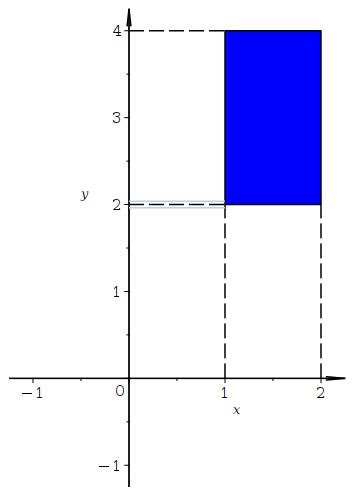
\includegraphics[width=0.25\paperwidth]{example.2.1}

Тепер застосуємо теорему про зведення кратного інтегралу до повторного:
\[
\iint\limits_{D}\left(x^2+y^2\right)d x d y = \int\limits_1^2\left(\int\limits_{2}^{4}\left(x^{2}+y^{2}\right)d y\right)dx.
\]
\begin{remark}
Можна було використати інший порядок змінних $x$ і $y$ і отримати
\[
\iint\limits_{D}\left(x^2+y^2\right)d x d y = \int\limits_{2}^{4}\left(\int\limits_1^2\left(x^{2}+y^{2}\right) d x\right)d y.
\]
В якості вправи пропонуємо підрахувати цей повторний інтеграл і переконатись, що відповідь буде така сама.
\end{remark}
Знайдемо спочатку $\int\limits_{2}^{4}\left(x^{2}+y^{2}\right)d y$. Нагадаємо властивість лінійності інтеграла Рімана:
\[
\int\limits_{a}^{b}\left(f(y)+g(y)\right)d y = \int\limits_{a}^{b}f(y)d y+\int\limits_{a}^{b}g(y)d y.
\]
Тут
\[
\begin{array}{cc}
f(y) = x^2 & \mbox{ --- не залежить від } y\mbox{, при інтегруванні вважається константою!}\\
g(y) = y^2 &
\end{array}
\]
\[
\int\limits_{2}^{4}\left(x^{2}+y^{2}\right)d y = \int\limits_{2}^{4}x^{2}d y+\int\limits_{2}^{4}y^{2}d y
\]

Для знаходження першого доданку ${\int\limits_{2}^{4}x^{2}d y}$ спочатку знайдемо первісну функції ${x^2}$ (яка не залежить від змінної $y$, тобто є в цьому інтегралі константою!):
\[
\int x^{2}d y = x^2 y + C,
\]
а потім скористаємось формулою Ньютона--Лейбніця:
\[
\int\limits_{2}^{4}x^{2}d y = x^2 y \biggr|_{y=2}^4 = 4 x^2 - 2 x^2 = 2 x^2.
\]
Для знаходження другого доданку ${\int\limits_{2}^{4}y^{2}d y}$ спочатку знайдемо первісну функції ${y^2}$:
\[
\int\limits_{2}^{4}y^{2}d y = \frac{y^3}{3} + C,
\]
а потім скористаємось формулою Ньютона--Лейбніця:
\[
\int\limits_{2}^{4}y^{2}d y = \frac{y^3}{3} \biggr|_{y=2}^4 = \frac{4^3}{3} - \frac{2^3}{3} = \frac{56}{3}.
\]
У підсумку,
\[
\int\limits_{2}^{4}\left(x^{2}+y^{2}\right)d y = \int\limits_{2}^{4}x^{2}d y+\int\limits_{2}^{4}y^{2}d y = 2 x^2 + \frac{56}{3}.
\]
Значить,
\[
\iint\limits_{D}\left(x^2+y^2\right)d x d y = \int\limits_1^2\left(\int\limits_{2}^{4}\left(x^{2}+y^{2}\right)d y\right)dx = \int\limits_1^2\left(2 x^2 + \frac{56}{3}\right)dx.
\]
Знайдемо останній інтеграл. Згідно з лінійністю інтеграла Рімана
\[
\int\limits_1^2\left(2 x^2 + \frac{56}{3}\right)dx = 2 \int\limits_1^2 x^2 d x + \frac{56}{3}\int\limits_1^2dx.
\]
Для знаходження першого доданку ${2\int\limits_1^2 x^2 d x}$ спочатку знайдемо первісну функції ${x^2}$ (тепер ми інтегруємо по змінній $x$, і тому ця функція не  є в цьому інтегралі константою):
\[
\int x^{2}d x = \frac{x^3}{3} + C,
\]
а потім скористаємось формулою Ньютона--Лейбніця:
\[
2\int\limits_{1}^{2}x^{2}d x = 2 \times\frac{x^3}{3} \biggr|_{1}^2 = 2\times \frac{2^3}{3} - 2\times \frac{1^3}{3} = \frac{14}{3}.
\]
Для знаходження другого доданку ${\frac{56}{3}\int\limits_1^2dx}$ спочатку знайдемо первісну константи ${1}$:
\[
\int\limits d x = x + C,
\]
а потім скористаємось формулою Ньютона--Лейбніця:
\[
\frac{56}{3}\int\limits_{1}^{2} d x = \frac{56}{3} x \biggr|_{1}^2 = \frac{56}{3}\times 2 - \frac{56}{3} \times 1 = \frac{56}{3}.
\]
У підсумку,
\[
\iint\limits_{D}\left(x^2+y^2\right)d x d y =  \int\limits_1^2\left(2 x^2 + \frac{56}{3}\right)dx = .\frac{14}{3} + \frac{56}{3} = \frac{70}{3}.
\]
Відповідь: ${\iint\limits_{D}\left(x^2+y^2\right)d x d y = .\frac{14}{3} + \frac{56}{3} = \frac{70}{3}.}$
\end{example}

\begin{example}
Знайти ${\iint\limits_{D}8 x^2 \sin\left(4 x y\right)d x d y}$, де через $D$ позначений пря\-мо\-кут\-ник ${D = \segment{\frac{\pi}{2}}{\pi}\times\segment{0}{1}}$.

Спочатку зробимо рисунок області інтегрування $D$.

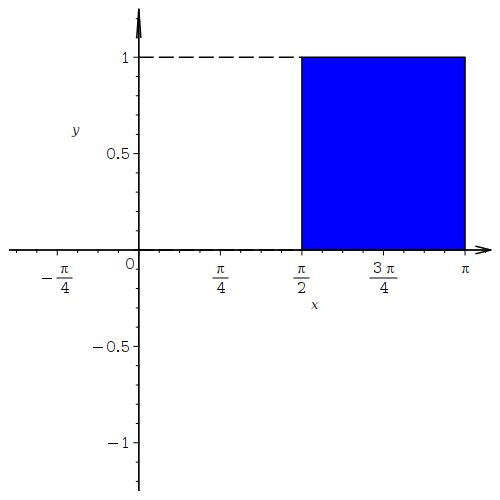
\includegraphics[width=0.25\paperwidth]{example.2.2}

Тепер застосуємо теорему про зведення кратного інтегралу до повторного:
\[
\iint\limits_{D}8 x^2 \sin(4 x y)d x d y = \int\limits_{\frac{\pi}{2}}^{\pi}\left(\int\limits_{0}^{1}8 x^2 \sin\left(4 x y\right)d y\right)dx.
\]

Знайдемо спочатку $\int\limits_{0}^{1}8 x^2 \sin\left(4 x y\right)d y$. Нагадаємо властивість лінійності інтеграла Рімана:
\[
\int\limits_{a}^{b}\alpha f(y) d y = \alpha \int\limits_{a}^{b}f(y)d y.
\]
Тут
\[
\begin{array}{cc}
f(y) =  \sin\left(4 x y\right) & \\
\alpha = 8 x^2  & \mbox{ --- не залежить від } y\mbox{, при інтегруванні вважається константою!}
\end{array}
\]
\[
\int\limits_{0}^{1}8 x^2 \sin\left(4 x y\right)d y = 8 x^2 \int\limits_{0}^{1} \sin\left(4 x y\right)d y.
\]
Тепер знайдемо первісну функції ${\sin\left(4 x y\right)}$:
\[
\int\limits \sin\left(4 x y\right)d y = -\frac{1}{4 x}\cos\left(4 x y\right) + C,
\]

а потім скористаємось формулою Ньютона--Лейбніця:
\[
\int\limits_{0}^1 \sin\left(4 x y\right)d y = -\frac{1}{4 x}\cos\left(4 x y\right) \biggr|_{y=0}^1 = -\frac{1}{4 x}\cos\left(4 x\right) - \left(-\frac{1}{4 x}\cos\left(0\right)\right) = \frac{1 - \cos \left(4 x\right)}{4 x}.
\]
У підсумку,
\[
\int\limits_{0}^{1}8 x^2 \sin\left(4 x y\right)d y = 8 x^2\times \frac{1 - \cos \left(4 x\right)}{4 x} = 2x \left(1 - \cos \left(4 x\right)\right).
\]
Значить,
\[
\iint\limits_{D}8 x^2 \sin(4 x y)d x d y = \int\limits_{\frac{\pi}{2}}^{\pi} 2x \left(1 - \cos \left(4 x\right)\right) d x.
\]
Знайдемо останній інтеграл. Для знаходження визначеного інтегралу
\[
\int\limits_{\frac{\pi}{2}}^{\pi} 2x \left(1 - \cos \left(4 x\right)\right) d x
\]
потрібно скористатись формулою інтегрування частинами:
\[
\int_a^b u d v = u v\biggr|_a^b - \int_a^b v d u.
\]
Тут
\[
\begin{array}{l}
u = 2 x, \\
d v = \left(1 - \cos \left(4 x\right)\right) d x.
\end{array}
\]
Для знаходження ${d u}$ потрібно продифференціювати (знайти похідну) ${u}$:
\[
d u  = \left(2 x \right)' d x = 2 d x,
\]
a для знаходження $v$ потрібно проінтегрувати ${d v}$:
\[
v = \int \left(1 - \cos \left(4 x\right)\right) d x \stackrel{{\normalfont\mbox{\tiny{(лінійність!})}}}{=} \int d x - \int \cos\left(4 x\right) d x = x - \frac{1}{4}\sin\left(4 x\right) + C.
\]
Таким чином,
\[
\begin{array}{l}
\int\limits_{\frac{\pi}{2}}^{\pi} 2x \left(1 - \cos \left(4 x\right)\right) d x = \left(2 x \left(x - \frac{1}{4}\sin\left(4 x\right)\right)\right)\biggr|_\frac{\pi}{2}^\pi - \int\limits_{\frac{\pi}{2}}^{\pi} \left(x - \frac{1}{4}\sin\left(4 x\right)\right) 2 d x = \\ =
\left(2 \pi \left(\pi - \frac{1}{4}\sin\left(4 \pi\right)\right)\right) - \left(2 \frac{\pi}{2} \left(\frac{\pi}{2} - \frac{1}{4}\sin\left(4\times \frac{\pi}{2}\right)\right)\right) - \int\limits_{\frac{\pi}{2}}^{\pi} \left(2x - \frac{1}{2}\sin\left(4 x\right)\right) d x = \\
=2\pi^2 - \frac{\pi^2}{2} - \int\limits_{\frac{\pi}{2}}^{\pi} \left(2x - \frac{1}{2}\sin\left(4 x\right)\right) d x = \frac{3\pi^2}{2} - \int\limits_{\frac{\pi}{2}}^{\pi} \left(2 x - \frac{1}{2}\sin\left(4 x\right)\right) d x.
\end{array}
\]
Для знаходження інтегралу ${\int\limits_{\frac{\pi}{2}}^{\pi} \left(2 x - \frac{1}{2}\sin\left(4 x\right)\right) d x}$ спочатку скористаємось лінійністю
\[
\int\limits_{\frac{\pi}{2}}^{\pi} \left(2 x - \frac{1}{2}\sin\left(4 x\right)\right) d x = 2\int\limits_{\frac{\pi}{2}}^{\pi} x d x - \frac{1}{2} \int\limits_{\frac{\pi}{2}}^{\pi} \sin\left(4 x\right) d x,
\]
потім знайдемо первісні функцій $x$ і $\sin\left(4 x\right)$
\[
\begin{array}{c}
\int x d x = \frac{x^2}{2} + C,\\
\int \sin\left(4 x\right) d x = -\frac{1}{4}\cos\left(4 x\right) + C,
\end{array}
\]
а потім скористаємось формулою Ньютона--Лейбніця:
\[
\begin{array}{c}
\int\limits_{\frac{\pi}{2}}^{\pi} x d x = \frac{x^2}{2}\biggr|_\frac{\pi}{2}^\pi = \frac{\pi^2}{2} - \frac{(\frac{\pi}{2})^2}{2} = \frac{\pi^2}{2} - \frac{\pi^2}{8} = \frac{3\pi^2}{8},\\
\int\limits_{\frac{\pi}{2}}^{\pi} \sin\left(4 x\right) d x = -\frac{1}{4}\cos\left(4 x\right)\biggr|_\frac{\pi}{2}^\pi = -\frac{1}{4}\cos\left(4 \pi\right) - \left(-\frac{1}{4}\cos\left(4 \times \frac{\pi}{2}\right)\right) = 0.
\end{array}
\]
У підсумку,
\[
\int\limits_{\frac{\pi}{2}}^{\pi} \left(2 x - \frac{1}{2}\sin\left(4 x\right)\right) d x = 2\int\limits_{\frac{\pi}{2}}^{\pi} x d x - \frac{1}{2} \int\limits_{\frac{\pi}{2}}^{\pi} \sin\left(4 x\right) d x = 2\times \frac{3\pi^2}{8} - \frac{1}{2} \times 0 = \frac{3\pi^2}{4},
\]
значить,
\[
\int\limits_{\frac{\pi}{2}}^{\pi} 2x \left(1 - \cos \left(4 x\right)\right) d x = \frac{3\pi^2}{2} - \frac{3\pi^2}{4} = \frac{3\pi^2}{4}.
\]
Остаточно,
\[
\iint\limits_{D}8 x^2 \sin(4 x y)d x d y = \frac{3\pi^2}{4}.
\]
Відповідь: ${\iint\limits_{D}8 x^2 \sin(4 x y)d x d y = \frac{3\pi^2}{4}.}$
\begin{remark}
В цьому прикладі ми також могли використати інший порядок змінних при зведенні до повторного інтегралу, і ми б отримали наступну рівність:
\[
\iint\limits_{D}8 x^2 \sin(4 x y)d x d y = \int\limits_{0}^{1}\left(\int\limits_{\frac{\pi}{2}}^{\pi}8 x^2 \sin\left(4 x y\right)d x\right)dy.
\]
Але в цьому випадку знаходження інтегралу всередині буде відносно складним і в результаті ми отримаємо
\[
\begin{array}{c}
\int\limits_{\frac{\pi}{2}}^{\pi}8 x^2 \sin\left(4 x y\right)d x = \\= -\dfrac{8 \pi^{2} y^{2} \cos \! \left(4 y \pi \right)-2 y^{2} \cos \! \left(2 y \pi \right) \pi^{2}-4 y \pi  \sin \! \left(4 y \pi \right)}{4 y^{3}}+\\
+\dfrac{2 y \sin \! \left(2 y \pi \right) \pi -\cos \! \left(4 y \pi \right)+\cos \! \left(2 y \pi \right)}{4 y^{3}}.
\end{array}
\]
Останній вираз потрібно буде ще проінтегрувати по $y$ від~$0$~до~$1$, що буде значно складніше наведеного розв'язання. Таким чином,

\fbox{
\begin{minipage}{0.7\textwidth}
\textbf{складність знаходження подвійного інтегралу може суттєво залежати від того, в якому порядку зводити його до повторного.}
\end{minipage}
}
\end{remark}
\end{example}
\begin{example}
Знайти ${\iiint\limits_{V}\left(x + y^2 - 2 z\right)d x d y d z}$, де через $V$ позначений пря\-мо\-кут\-ний паралелепіпед ${V = \segment{1}{2}\times\segment{1}{3}\times\segment{4}{5}}$.
Застосуємо теорему про зведення кратного інтегралу до повторного:
\[
\iiint\limits_{V}\left(x + y^2 - 2 z\right)d x d y d z = \int\limits_1^2\left(\int\limits_1^3\left(\int\limits_4^5\left(x + y^2 - 2 z\right)d z\right)d y\right)d x.
\]

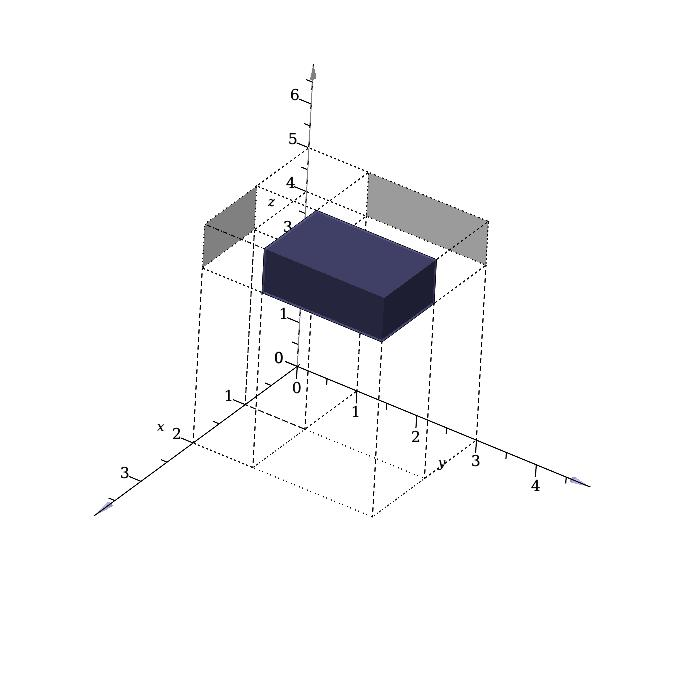
\includegraphics[width=0.5\paperwidth]{example.2.3}

Знайдемо спочатку ${\int\limits_4^5\left(x + y^2 - 2 z\right)d z}$. З лінійності інтеграла Рімана випливає, що
\[
\int\limits_4^5\left(x + y^2 - 2 z\right)d z = \int\limits_4^5xd z + \int\limits_4^5y^2d z - 2 \int\limits_4^5 zd z.
\]
Тепер знайдемо первісні відповідних функцій (пам'таємо, що інтегрування відбувається по змінній $z$, тому змінні $x$ та $y$ при цьому є константами):
\[
\begin{array}{c}
\int x d z = x z + C,\\
\int y^2 d z = y^2 z + C,\\
\int z d z = \frac{z^2}{2} + C,
\end{array}
\]

а потім скористаємось формулою Ньютона--Лейбніця:
\[
\begin{array}{c}
\int\limits_4^5 x d z = x z\biggr|_{z=4}^5 = 5 x - 4 x = x,\\
\int\limits_4^5 y^2 d z = y^2 z\biggr|_{z=4}^5 = 5 y^2 -4 y^2 = y^2,\\
\int\limits_4^5 z d z = \frac{z^2}{2}\biggr|_{z=4}^5 = \frac{25}{2} - \frac{16}{2} = \frac{9}{2},
\end{array}
\]
Таким чином,
\[
\int\limits_4^5\left(x + y^2 - 2 z\right)d z = x + y^2 - 2 \times .\frac{9}{2} = x + y^2 -9
\]
і
\[
\iiint\limits_{V}\left(x + y^2 - 2 z\right)d x d y d z = \int\limits_1^2\left(\int\limits_1^3\left(x + y^2 -9\right)d y\right)d x.
\]
Тепер шукаємо
\[
\int\limits_1^3\left(x + y^2 -9\right)d y \stackrel{{\normalfont\mbox{(лінійність)}}}{=} \int\limits_1^3 x d y  + \int\limits_1^3 y^2d y  - 9 \int\limits_1^3 d y.
\]
Тепер знайдемо первісні відповідних функцій (пам'таємо, що інтегрування відбувається по змінній $y$, тому змінна $x$ при цьому є константою):
\[
\begin{array}{c}
\int x d y = x y + C,\\
\int y^2 d y = \frac{y^3}{3} + C,\\
\int d y = y + C,
\end{array}
\]

а потім скористаємось формулою Ньютона--Лейбніця:
\[
\begin{array}{c}
\int\limits_1^3 x d y = x y\biggr|_{y=1}^3 = 3 x - x = 2 x,\\
\int\limits_1^3 y^2 d y = \frac{y^3}{3}\biggr|_{y=1}^3 = \frac{3^3}{3} - \frac{1^3}{3} = \frac{26}{3},\\
\int\limits_1^3 d y = y\biggr|_{y=1}^3 = 3 - 1 = 2.
\end{array}
\]
Далі
\[
\int\limits_1^3\left(x + y^2 -9\right)d y = 2 x  +\frac{26}{3} - 9 \times 2 = 2 x - \frac{28}{3}.
\]
і
\[
\iiint\limits_{V}\left(x + y^2 - 2 z\right)d x d y d z = \int\limits_1^2\left(2 x - \frac{28}{3}\right)d x.
\]
Знайдемо останній інтеграл.
\[
\int\limits_1^2\left(2 x - \frac{28}{3}\right)d x \stackrel{{\normalfont\mbox{(лінійність)}}}{=} 2 \int\limits_1^2 x d x - \frac{28}{3} \int\limits_1^2 d x.
\]
Первісні:
\[
\begin{array}{c}
\int x d x = \frac{x^2}{2} + c,\\
\int d x  = x + C.
\end{array}
\]
Тепер формула Ньютона--Лейбніця:
\[
\begin{array}{c}
\int x d x = \frac{x^2}{2}\biggr|_{1}^2 = \frac{2^2}{1} - \frac{1^2}{2} = \frac{3}{2},\\
\int d x  = x \biggr|_{1}^2 = 2 - 1 = 1,\\
\end{array}
\]
Остаточно,
\[
\iiint\limits_{V}\left(x + y^2 - 2 z\right)d x d y d z = 2 \times \frac{3}{2}- \frac{28}{3} \times 1 = -\frac{19}{3}.
\]
Відповідь: ${-\frac{19}{3}}$.
\end{example}
\nocite{Gar84}

